\section{Static Information Flow Analysis} \label{sect:design}
%
\subsection{A Simple Example}

While TrustZone technology in Armv8-M processors offers robust security measures, it remains susceptible to side channel attacks due to secret-dependent control flow, resulting in observable timing variations or secret-dependent memory access patterns \cite{armdeveloper}. Furthermore, it's worth noting that TrustZone might not entirely mitigate implicit and explicit information leaks resulting from unintentional developer errors in secure coding practices, system architecture flaws, and non-compliance with stringent security standards and protocols.

To elaborate, consider a secure One-Time Password (\gls{OTP}) system illustrated in Fig. \ref{fig:OTP}. \gls{OTP} system is integral in verifying mobile users accessing critical web services that require a heightened level of security. An \gls{OTP} is a dynamically generated numeric or alphanumeric string of characters used to authenticate a user for a single transaction or session with an authentication server. This approach augments the traditional user ID and password authentication by introducing a dynamic password that changes with each authentication attempt. The \gls{OTP} mechanism operates by generating a code using an internal clock (or counter) and a factory-encoded secret key known as the 'seed.' 

To maintain the confidentiality of both the generated \gls{OTP}s and the associated seeds, the code and data involved in \gls{OTP} operations inhabit a secure enclave within TrustZone \cite{trustotp}. This enclave establishes a isolated space, distinct from the regular operating system running in the normal world. TrustZone technology guarantees the integrity and confidentiality of \gls{OTP}s and seeds by restricting access exclusively to the secure domain.

However, any inadvertent mishandling of the seeds or \gls{OTP}s—such as storing them in plaintext on unprotected memory, logging them, or exposed via non-secure I/O —or if an implicit flow is triggered by updating a publicly observable variable within the program control flow—an attacker could potentially access the generated \gls{OTP}s. Furthermore, the attacker might deduce secrets by analyzing time variations within a secret-dependent branch.

\begin{figure}
  \centering
  \medskip
  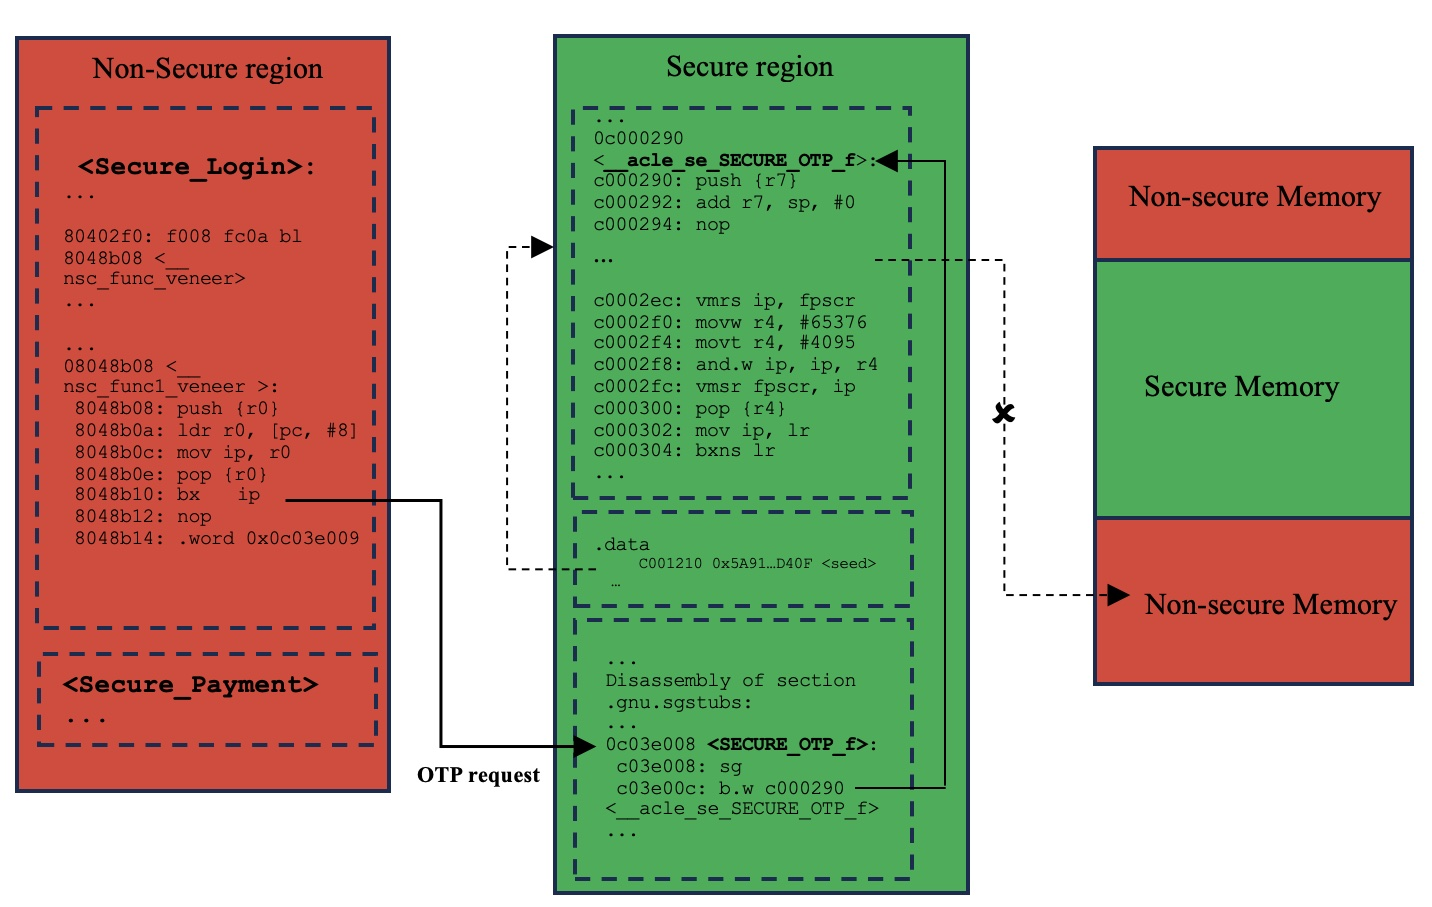
\includegraphics[width=.9\textwidth]{chapters/chapter3/image/OTP.jpg}
  \caption[Short caption for Table of Figures]{TrustZone-based Implementation of Secure OTP Generation}
  \label{fig:OTP}
\end{figure}

We present an approach that merges taint tracking techniques with symbolic execution of trusted application (\gls{TA}) binaries to systematically identify the undesired information leakage. Subsequently, we notify developers and designers of these identified leakage points for further action and resolution. 

\subsection{Scope and Threat Model}

\textit{Scope.} Our focus revolves around small-scale embedded systems and IoT devices that operate using MCUs, such as the Arm Cortex-M family. These MCUs operate within strict constraints, characterized by limited computing power and memory. They feature simplified microarchitectures, lacking components like caches and typically operating with 2-3 pipeline stages. Additionally, they do not support virtual memory. Generally, MCUs consist of a single CPU while offering a diverse array of peripherals, including UART, SPI, timers, DMAs, and I2C, among others. Some devices may incorporate MPUs, and the latest iterations of Armv8-M MCUs introduce support for dual security states, namely secure and non-secure worlds (known as TrustZone-M). These MCUs are engineered to ensure highly predictable outcomes, consistently delivering identical outputs for specific inputs within defined timing constraints.

\textit{Threat model.} The adversary’s goal is to extract sensitive information from an isolated environment by bypassing the memory isolation security mechanisms in TrustZone. We assume the attacker has access to either the source code or compiled binary code of the victim's program. Additionally, they can monitor the program's execution time and outputs. Furthermore, we consider a more capable attacker who has complete control over the unprotected normal world and its resources. This includes the ability to manage bus masters (e.g., DMA), configure peripherals like timers, and control scheduling decisions. We are not considering side channels arising from cache contention or branch prediction feature, as they fall beyond the scope of this work due to their absence in the targeted MCU architecture.

\subsection{Taint Tracking of Function Inputs}

Our method involves an information flow analysis that links each value with a security tag indicating its sensitivity level. We primarily categorize these levels into two labels: '\textit{H}' for high sensitivity and '\textit{L}' for low sensitivity, where '\textit{H}' signifies higher sensitivity than '\textit{L}'. Each input (initial state of registers, etc.) and output (final state of registers, etc.) of a program is assigned one of these labels. To effectively track and identify both explicit and implicit data flows of high sensitivity during program execution, our approach incorporates an effective symbolic taint-tracking mechanism.

Specifically, initial register contents and associated memory are transparently substituted with unconstrained symbolic values. We, furthermore, utilize Angr\footnote{https://angr.io/}’s annotation system to flag highly sensitive symbolic values as tainted. This taint, conservatively propagated throughout symbolic execution, allows for convenient querying during subsequent analysis to identify potential information leakage. 

\subsection{Timing-Sensitive Information Flow Policy}

An information-flow analysis verifies the absence of undesired information leakage within a program. A timing-sensitive variant of this analysis considers the impact of confidential data on the program's execution time. The intended security assurance is typically defined through information flow policies that prevent secret data from affecting an attacker's observations. This study utilizes a symbolic taint-tracking strategy to monitor potential policy violations during execution.

To this end, taint tags follow Angr's propagation rules during symbolic program execution, aligning with ARMv8-M instruction semantics. For example, in the case of an instruction like ‘ADD dst, src1, src2’, a taint propagation rule might dictate that the resulting tag of 'dst' is determined by performing a bit-wise OR operation on the tags of ‘src1’ and ‘src2’. Specifically, these rules imposes constraints on the sensitivity of data stored in registers and memory cells throughout program execution, affecting their state upon program termination. 

\subsection{Detection of timing side channels}

To ensure the absence of timing side channels within a program, our approach involves the initial computation of control-dependence regions for each branch instruction dependent on secret data. This computation employs the Safe Over-Approximation Properties (SOAPs) as defined in \cite{MantelAVR}. In particular, our focus lies in comparing the execution times between the 'then' and 'else' branches, distinguishing two distinct control-dependence regions for jumps influenced by confidential information.

Afterward, we sums up the execution time of all instructions within each region following the \textit{Definition} \ref{def:timing}. In scenarios where a nested branch \textit{br1} exists within the region of another branch \textit{br0}, a recursive procedure becomes necessary due to only one path of \textit{br1} being executed, whereas the positive part of \textit{Definition} \ref{def:timing} accounts for both paths' cumulative execution time. We address this by subtracting the execution time of the 'then' branch of \textit{br1}.

\newtheorem{definition}{Definition}[section]
\begin{definition}\label{def:timing}
    The function \textbf{branchPathTime\textsuperscript{r}} is defined recursively as: \\
    
   \centerline{$branchPathTime^r(br) := \Sigma (execution\_time(ins) - branchPathTime^{then}(ins))$}

   Where:
\begin{align*}
& \bullet \quad r \in \{ \text{then}, \text{else} \} \\
& \bullet \quad br \in \{ \text{beq}, \text{bne}, \text{bgt}, \text{blt}, \text{bge}, \text{ble} \} \\
& \bullet \quad \forall \text{ins} \in \text{region}^r(br)
\end{align*}

\end{definition}

Within ARMv8-M architecture, conditional branch instructions require an extra clock cycle when they are taken. With this fact, if the total time required for executing the 'then' region plus one equals the time taken for jumping and executing the 'else' region in a secret-dependent branch, it becomes impossible to discern the value of secret data by observing the program's overall execution time.

Furthermore, identifying the Nemesis vulnerability in an ARMv8-M binary involves pinpointing a jump instruction depending on secret data. Due to the variable execution times of branch instructions in ARMv8-M architecture when taken or not, an attacker can interrupt a branch instruction to capture the secret information. Consequently, the attacker can even execute a Nemesis attack on balanced paths.

To detect the BUSted vulnerability in a binary, we meticulously traverse every path within a branch dependent on secret information, scrutinizing the execution points of 'str' or 'ldr' instructions. If these instructions execute at different clock offsets on conditional paths, it exposes a potential vulnerability for attackers to exploit distinct memory access patterns and gain access to sensitive information.

\subsection{Augmented Taint Flow Directives}

Secret-dependent branches introduce variations in the program flow based on confidential information. By observing changes in execution time, logical operations, or other side channel information arising from these branches, attackers can deduce details about the secret data, such as its value or structure. Consequently, when a secret-dependent branch involves an operation where a memory cell or register is written within a particular path, it's crucial to mark that register or memory as tainted. These elements carry highly sensitive information during program execution, causing variations that attackers can exploit to infer the secret.

We employ Angr’s MemoryMixin extension, which conducts exhaustive validations on every memory access. Specifically, when these accesses occur within secret-dependent branches, we annotate the potentially symbolic values as tainted to reflect their elevated sensitivity within that particular context. This approach guarantees the absence of flows from secret information to attacker-observable outputs.
